\begin{frame}
\begin{example}
Where is this function defined?
\begin{columns}[c]
\column{.4\textwidth}
\[
f(x) = \frac{x^2 - x - 2}{\alertNoH{3}{x - 2}}
\]
\ \uncover<4->{
\psset{xunit=0.8cm, yunit=0.8cm}
\begin{pspicture}(-3, -2)(3,4)
 \psframe*[linecolor=white](-3,-2)(3,4) \psaxes[labels=none]{<->}(0,0)(-3,-2)(3,4)
 \psplot[linecolor=red, plotpoints=1000]{-3}{3}{x 1 add }
 \fcHollowDot{2}{3}
\end{pspicture} %
%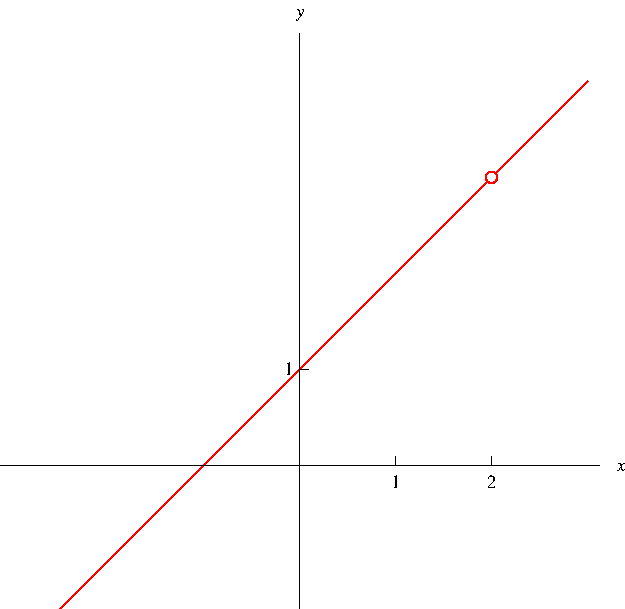
\includegraphics[height=4.5cm]{continuity/pictures/02-05-ex2a.pdf}%
}
\column{.6\textwidth}
\begin{itemize}
\item<2-| alert@2-3>  $f(2)$ \fcAnswer{3}{is not defined.}
%\item<4->  Discontinuous at 2. %Todor: I disagree: the function is not defined at 2, rather than discontinuous.
\item<4->  This is called a removable discontinuity because we could extend the definition of $f$ to $2$ to make $f$ defined and continuous at that point.
\end{itemize}
\end{columns}
\end{example}
\end{frame}